%===============================================================
% Template using official colors of Czech Technical University.
% They are defined by new graphical manual - 2017.
% Specially designed for Laboratory of Structure of Biomolecules
% Share and modify as you like. Keep the name of the author.
% It is forbidden to use the template commercially.
% Author: Martin Malý.
% Published: 23.9.2017.
%===============================================================

\documentclass{beamer}
\usepackage[utf8]{inputenc}

\usetheme{Madrid}
  
\definecolor{cvut_navy}{HTML}{0065BD}
\definecolor{cvut_blue}{HTML}{6AADE4}
\definecolor{cvut_gray}{HTML}{156570}

\setbeamercolor{section in toc}{fg=black,bg=white}
\setbeamercolor{alerted text}{fg=cvut_blue}
\setbeamercolor*{palette primary}{bg=cvut_navy,fg=gray!20!white}
\setbeamercolor*{palette secondary}{bg=cvut_blue,fg=white}
\setbeamercolor*{palette tertiary}{parent=palette primary}
\setbeamercolor*{palette quaternary}{fg=green,bg=gray!5!white}

\setbeamercolor*{sidebar}{fg=cvut_navy,bg=gray!15!white}


\setbeamercolor{titlelike}{parent=palette primary}
\setbeamercolor{frametitle}{parent=palette primary}

\setbeamercolor*{separation line}{}
\setbeamercolor*{fine separation line}{}

\setbeamertemplate{navigation symbols}{} 


\usepackage{eqnarray,amsmath}
\usepackage{amsfonts}
\usepackage{amssymb}
\usepackage{graphicx}
\usepackage{lmodern} % pro pismo tucne a zaroven kurziva
\usepackage{bm} % pro pismo tucne a zaroven kurziva
\usepackage{epstopdf}
\usepackage{changepage}
\usepackage{array,booktabs}
  
\usepackage{subcaption}
\usepackage{animate}
\usepackage[linesnumbered,ruled,vlined]{algorithm2e}

% definice makra pro české uvozovky:
\def\bq{\mbox{\kern.1ex\protect\raisebox{-1.3ex}[0pt][0pt]{''}\kern-.1ex}}
\def\eq{\mbox{\kern-.1ex``\kern.1ex}}
\def\ifundefined#1{\expandafter\ifx\csname#1\endcsname\relax }%
\ifundefined{uv}%
        \gdef\uv#1{\bq #1\eq}
\fi
% konec .... použití makra pro psaní český uvozovek: \uv{text uvnitř uvozovek}

%====================================================
%========== DEFINITION OF AUTHORS ETC...=============
%====================================================
\author[Artyom Tsoy]{Artyom Tsoy}
\institute[]{Czech Technical University in Prague \\ 
Faculty of Electrical Engineering\\
Department of Cybernetics\\
\vspace{2mm}supervisor: Ing. Vojtěch Vonásek, Ph.D.}
\title[Bachelor thesis]{Improving Path Planning Methods Using Machine Learning}
% \subtitle{subtitle}
\date[]{12.06.2024}

%====================================================
%========== BEGINNING OF DOCUMENT ===================
%====================================================
\begin{document}

\begin{frame}
	\titlepage
	\begin{center}
  		\includegraphics[height=1.3cm]{files/symbol_cvut_plna_samostatna_verze.pdf}
	\end{center}
\end{frame}


\logo{\includegraphics[height=1cm]{files/symbol_cvut_plna_samostatna_verze.pdf}}


% % ==========================================================================
% \begin{frame}
% 	\frametitle{Introduction}	
% 	\begin{figure}[!ht]
% 		\centering
% 		\begin{subfigure}[b]{0.55\textwidth}
% 			\includegraphics[width=\textwidth]{figChap1/The-piano-movers-problem-EET.png}
% 		\end{subfigure}
% 		\caption{The Piano Movers Problem. Image courtesy of~\cite{rickert2014piano}.}%\label{fig:animals}
% 	  \end{figure}
% \end{frame}
% % ==========================================================================

% ==========================================================================
\begin{frame}
	\frametitle{Introduction}	
	\begin{figure}[!ht]
		\centering
		\begin{subfigure}[b]{0.3\textwidth}
			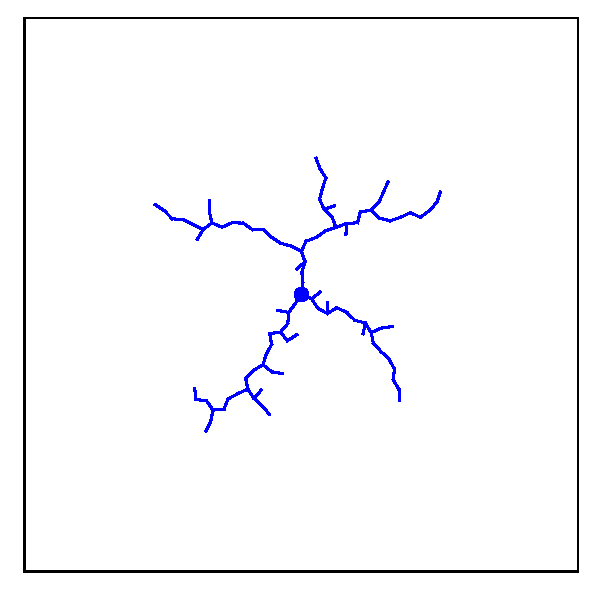
\includegraphics[width=\textwidth]{figChap3/2RRTexpansion100.eps}
			\caption{100 iterations}
			% \label{fig:gull}
		\end{subfigure}
		~ %add desired spacing between images, e. g. ~, \quad, \qquad, \hfill etc. 
		  %(or a blank line to force the subfigure onto a new line)
		\begin{subfigure}[b]{0.3\textwidth}
			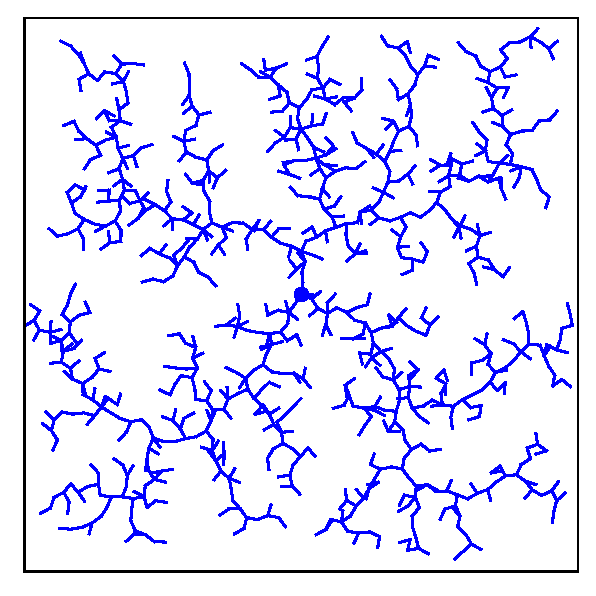
\includegraphics[width=\textwidth]{figChap3/2RRTexpansion1000.eps}
			\caption{1000 iterations}
			% \label{fig:tiger}
		\end{subfigure}
		~ %add desired spacing between images, e. g. ~, \quad, \qquad, \hfill etc. 
		%(or a blank line to force the subfigure onto a new line)
		\begin{subfigure}[b]{0.3\textwidth}
			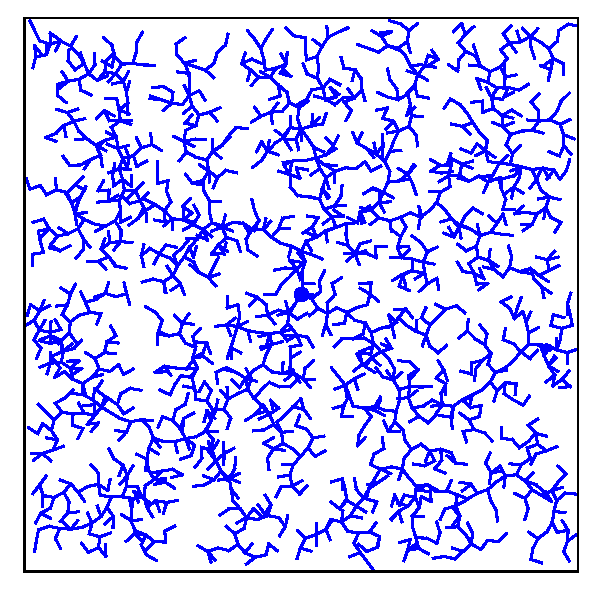
\includegraphics[width=\textwidth]{figChap3/2RRTexpansion2000.eps}
			\caption{2000 iterations}
			% \label{fig:mouse}
		\end{subfigure}
		\caption{Example of RRT expansion in 2D $\mathcal{C}$-space.}
		\label{fig:RRTgrowing}
	  \end{figure} 
\end{frame}	
% ==========================================================================

% ==========================================================================
\begin{frame}
	\frametitle{Introduction}	
	\begin{figure}[!ht]
		\centering  
		\begin{subfigure}[b]{0.45\textwidth}
			\includegraphics[width=\textwidth]{figChap3/RRT_maze7748i119w.pdf}
			\caption{RRT.} 
		\end{subfigure}
		\begin{subfigure}[b]{0.45\textwidth}
			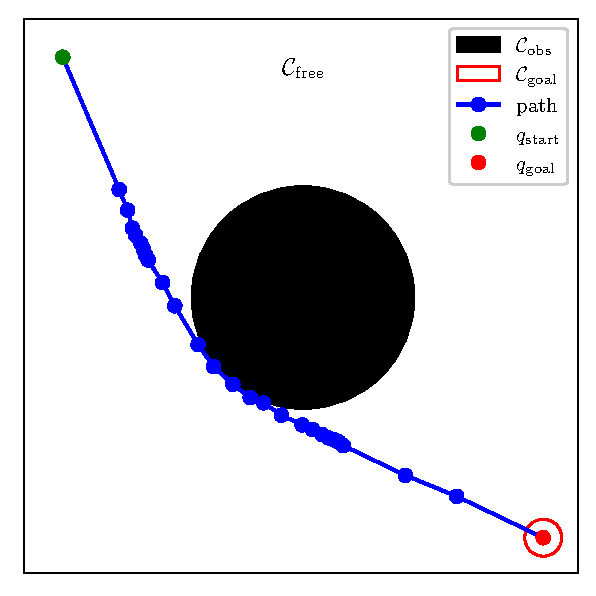
\includegraphics[width=\linewidth]{figChap2/ConfigSpace.eps}
			\caption{2D workspace with a 2D $\mathcal{C}$-space.}
		\end{subfigure} 
		\caption{RRT and a worspace example.} 
	  \end{figure}
\end{frame}	
% ==========================================================================


% % ==========================================================================
% \begin{frame}
% 	\frametitle{Introduction}	
% 	\begin{figure}
% 		\centering
% 		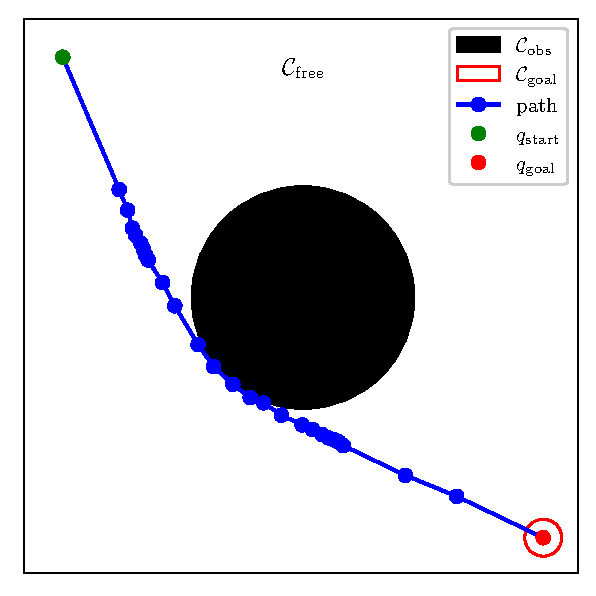
\includegraphics[width=0.5\linewidth]{figChap2/ConfigSpace.eps}
% 		\caption{2D workspace with a 2D $\mathcal{C}$-space.}
% 		\label{fig:config_space} 
% 	  \end{figure} 
% \end{frame}
% % ==========================================================================

% % ==========================================================================
% \begin{frame}
% 	\frametitle{RRT and RRT*}	
% 	\begin{figure}[!ht]
% 		\centering
% 		\begin{subfigure}[b]{0.45\textwidth}
% 			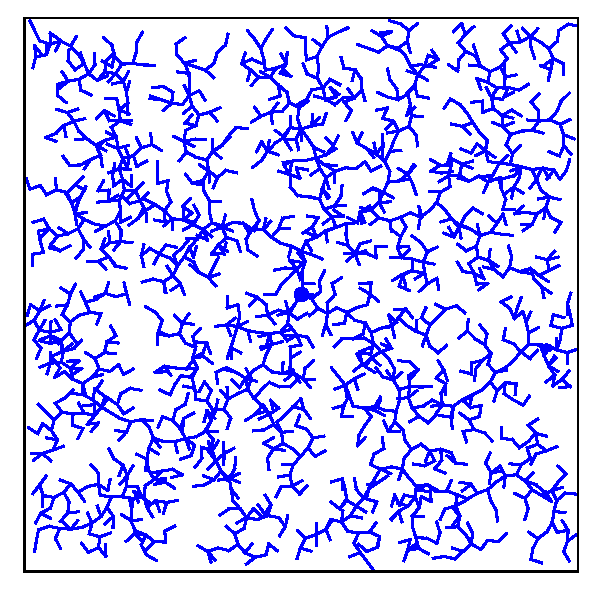
\includegraphics[width=\textwidth]{figChap3/2RRTexpansion2000.eps}
% 			\caption{RRT.}
% 			\label{fig:rrt2k}
% 		\end{subfigure}
% 		~ %add desired spacing between images, e. g. ~, \quad, \qquad, \hfill etc. 
% 		  %(or a blank line to force the subfigure onto a new line)
% 		\begin{subfigure}[b]{0.45\textwidth}
% 			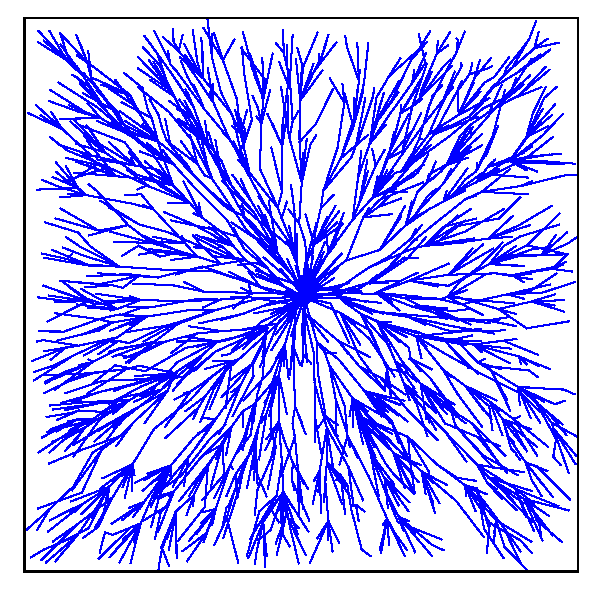
\includegraphics[width=\textwidth]{figChap3/RRTstar_expansion2000.eps}
% 			\caption{RRT*.}
% 			\label{fig:rrtstar2k}
% 		\end{subfigure}    
% 		\caption{RRT and RRT* comparison.}
% 		\label{fig:RRTvsRRTstar}
% 	  \end{figure}
% \end{frame}		
% % ==========================================================================

% % ==========================================================================
% \begin{frame}
% 	\frametitle{RRT and RRT*}	
% 	\begin{figure}[!ht]
% 		\centering 
% 		\begin{subfigure}[b]{0.45\textwidth}
% 			\includegraphics[width=\textwidth]{figChap3/RRT_maze7748i119w.pdf}
% 			\caption{RRT.} 
% 		\end{subfigure}
% 		~ %add desired spacing between images, e. g. ~, \quad, \qquad, \hfill etc.   
% 		  %(or a blank line to force the subfigure onto a new line)
% 		\begin{subfigure}[b]{0.45\textwidth}
% 			\includegraphics[width=\textwidth]{figChap3/RRTstar_maze_7060i_35w.pdf}
% 			\caption{RRT*.} 
% 		\end{subfigure}   
% 		\caption{RRT and RRT* comparison.} 
% 	  \end{figure}
% \end{frame}	
% % ==========================================================================

% ==========================================================================
\begin{frame}
	\frametitle{Motivation}	
	\noindent
	\begin{minipage}[t]{0.49\textwidth}
	  \vspace{0pt}
	  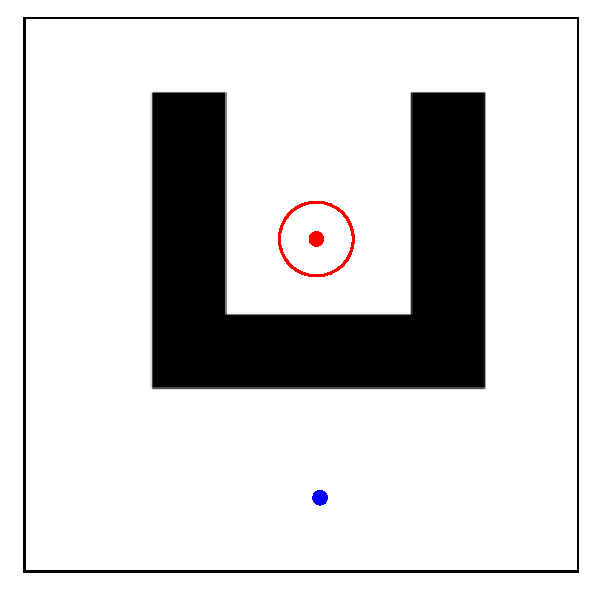
\includegraphics[width=\textwidth]{figChap4/SimpleMaze.eps} 
	  \captionof{figure}{An example of the 2D workspace with a 2D $\mathcal{C}$-space.}
	\end{minipage}
	\hfill
	\begin{minipage}[t]{0.49\textwidth}
	  \vspace{0.5cm}
	  \vfill
    \begin{center} % Center horizontally
      \begin{itemize}
        \item Efficient exploration of the \(\mathcal{C}\)-space;
        \vspace{0.2cm}
        \item Sampling points in \(\mathcal{C}_\text{free}\);
        \vspace{0.2cm}
		\item Real-time learning;
        \vspace{0.2cm}
		\item Finding better solutions with the same number of iterations.
		\vspace{0.2cm}
		\item Inspired by the work of~\cite{arslan2015machine}.
      \end{itemize}
    \end{center}
    \vfill
	\end{minipage}
  \end{frame}
% ==========================================================================

% ==========================================================================
\begin{frame}
	\frametitle{Proposed solution}	 
	\[ \hat{f}_\mathcal{X}(x) = \frac{1}{m} \sum_{i=1}^{m} K \left( x - x_{i} \right)\]
	\[K(x) = (2\pi)^{-\frac{d}{2}} \cdot \det(\textbf{H})^{-\frac{1}{2}} \cdot e^{-\frac{1}{2} x^T H^{-1} x}
\] 
\[
  P(y|x) = \frac{P(x|y) \cdot P(y)}{P(x)}
\] 
\[ P(x|y=1) = \hat{f}_{\mathcal{X}_{\text{obs}}}(x) = \frac{1}{|\mathcal{X}_{\text{obs}}|} \sum_{x' \in \mathcal{X}_{\text{obs}}} K \left( x - x' \right) \]
\[ P(x|y=0) = \hat{f}_{\mathcal{X}_{\text{free}}}(x) = \frac{1}{|\mathcal{X}_{\text{free}}|} \sum_{x' \in \mathcal{X}_{\text{free}}} K \left( x - x' \right) \]
\[ P(y=1) = \frac{|\mathcal{X}_{\text{obs}}|}{|\mathcal{X}_{\text{obs}}|+|\mathcal{X}_{\text{free}}|};\enspace
P(y=0) = \frac{|\mathcal{X}_{\text{free}}|}{|\mathcal{X}_{\text{obs}}|+|\mathcal{X}_{\text{free}}|}\]
\end{frame}	
% ==========================================================================


% ==========================================================================
\begin{frame}
	\frametitle{Proposed solution}	
	\begin{figure}[!ht]
		\centering 
		\begin{subfigure}[b]{1\textwidth}
			\includegraphics[width=\textwidth]{figChap4/GKDE_obsU.pdf} 
		\end{subfigure}   
		\caption{Obstacle density.} 
	  \end{figure}
\end{frame}	
% ==========================================================================

% ==========================================================================
\begin{frame}
	\frametitle{Proposed solution}	
	\begin{figure}[!ht]
		\centering  
		\begin{subfigure}[b]{1\textwidth}
			\includegraphics[width=\textwidth]{figChap4/GKDE_freeU.pdf} 
		\end{subfigure}
		\caption{Obstacle-free density.} 
	  \end{figure}
\end{frame}	
% ==========================================================================

% ==========================================================================
\begin{frame}
    \frametitle{Proposed Solution}
     
    \hspace*{2cm}    % Horizontal space to shift the pseudocode to the right
    \begin{minipage}{0.75\textwidth} % Adjust the width of the minipage as needed
        \centering
        \begin{algorithm}[H]
            \fontsize{8}{9}\selectfont   % Adjust the font size
            \caption{Sample Density}
            \label{alg:sample_density}
            \KwData{$\mathcal{X}_{\text{obs}}$, $\mathcal{X}_{\text{free}}$}
            \KwResult{Predicted sampled point $x$}
            \vspace{0.1cm}
            \hrule
            \vspace{0.2cm}
            $\gamma_{\text{free}} \gets 0$\;
            $\gamma_{\text{obs}} \gets 1$\; 
            \While{$\gamma_{\text{free}} < \gamma_{\text{obs}}$}{
              $x_{\text{rand}} \gets$ RandomConfiguration()\;
              $P_{\text{free}} \gets \frac{|\mathcal{X}_{\text{free}}|}{|\mathcal{X}_{\text{free}}| + |\mathcal{X}_{\text{obs}}|}$\;
              $P_{\text{obs}} \gets 1 - P_{\text{free}}$\;
              $b_{\text{free}} \gets$ DensityEstimator($x_{\text{rand}}$, $\mathcal{X}_{\text{free}}$)\;
              $b_{\text{obs}} \gets$ DensityEstimator($x_{\text{rand}}$, $\mathcal{X}_{\text{obs}}$)\;
              $\gamma_{\text{free}} \gets b_{\text{free}} \cdot P_{\text{free}}$\;
              $\gamma_{\text{obs}} \gets b_{\text{obs}} \cdot P_{\text{obs}}$\; 
            }
            $x \gets x_{\text{rand}}$\;
            \Return $x$\;
        \end{algorithm}
    \end{minipage}
    \vspace*{\fill} % Vertical space to center the pseudocode vertically
    
\end{frame}
% ==========================================================================

% ==========================================================================
\begin{frame}
    \frametitle{Proposed Solution}
     
    \begin{figure}[!ht]
		\centering
		\begin{subfigure}[b]{0.3\textwidth}
			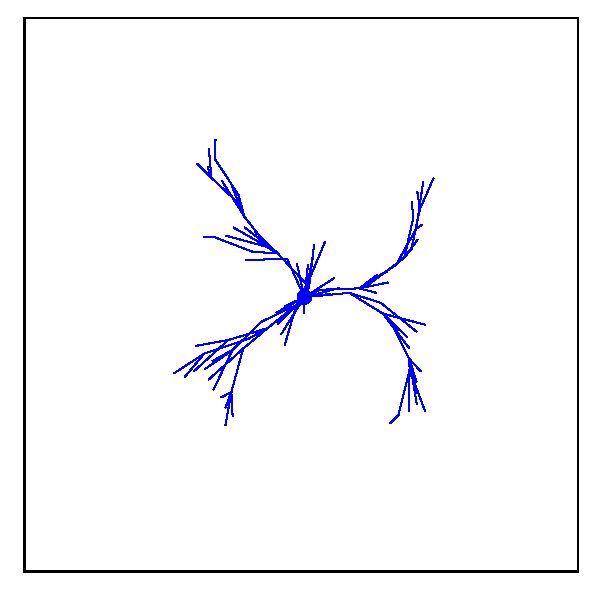
\includegraphics[width=\textwidth]{figChap3/RRTstar_expansion100.eps}
			\caption{100 iterations}
			% \label{fig:gull}
		\end{subfigure}
		~ %add desired spacing between images, e. g. ~, \quad, \qquad, \hfill etc. 
		  %(or a blank line to force the subfigure onto a new line)
		\begin{subfigure}[b]{0.3\textwidth}
			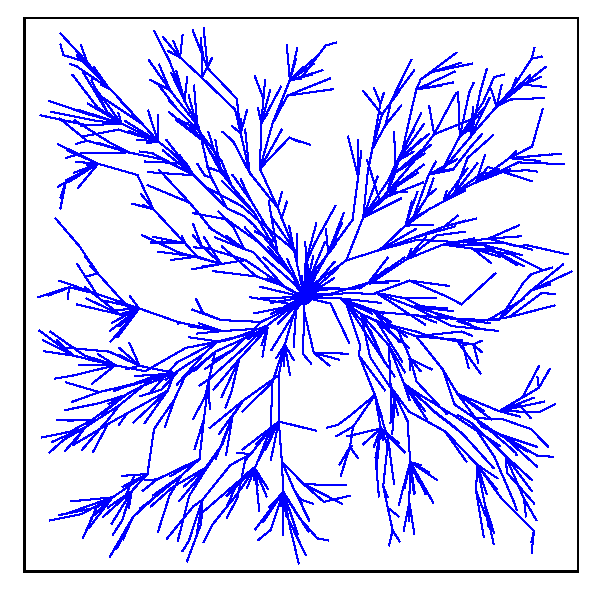
\includegraphics[width=\textwidth]{figChap3/RRTstar_expansion1000.eps}
			\caption{1000 iterations}
			% \label{fig:tiger}
		\end{subfigure}
		~ %add desired spacing between images, e. g. ~, \quad, \qquad, \hfill etc. 
		%(or a blank line to force the subfigure onto a new line)
		\begin{subfigure}[b]{0.302\textwidth}
			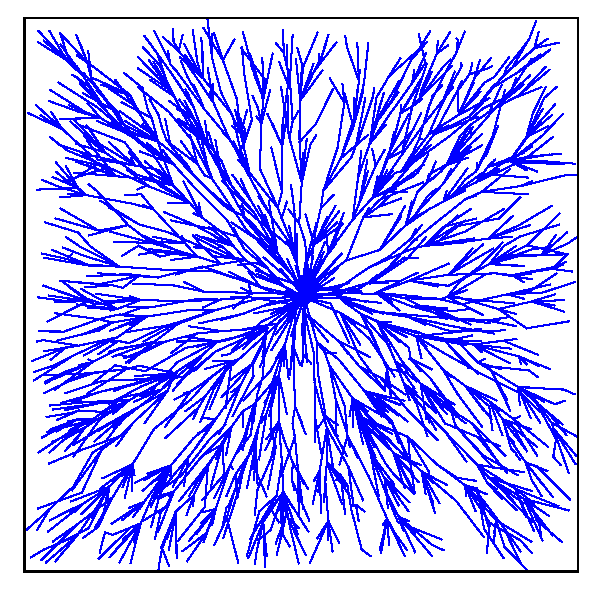
\includegraphics[width=\textwidth]{figChap3/RRTstar_expansion2000.eps}
			\caption{2000 iterations}
			% \label{fig:mouse}
		\end{subfigure}
		\caption{Example of RRT* expansion in 2D $\mathcal{C}$-space.}
		\label{fig:RRTstargrowing}
	  \end{figure}
    
\end{frame}
% ==========================================================================

% ==========================================================================
\begin{frame}
	\frametitle{Proposed solution}	
	\begin{figure}[!ht]
		\centering 
		\begin{subfigure}[b]{0.45\textwidth}
			\includegraphics[width=\textwidth]{figChap4/RRTstar_maze216.0.pdf}
			\caption{RRT* (216 u.d).}
			\label{fig:rrtstar_maze}
		\end{subfigure}  
		\begin{subfigure}[b]{0.45\textwidth}
			\includegraphics[width=\textwidth]{figChap4/RRTstarML_maze206.0.pdf}
			\caption{Improved RRT* (206 u.d).}
			\label{fig:rrtstarML_maze}
		\end{subfigure}
		\caption{RRT* and Improved RRT* comparison.}
		\label{fig:RRTstar_vs_RRTstarML}
	  \end{figure}
\end{frame}	
% ==========================================================================

% ==========================================================================
\begin{frame}
	\frametitle{Proposed solution}	
	\begin{figure}[!ht]
		\centering 
		\begin{subfigure}[b]{0.45\textwidth}
			\includegraphics[width=\textwidth]{figChap4/RRTstarML_learning206.0.pdf}
			 
		\end{subfigure}  
		\begin{subfigure}[b]{0.45\textwidth}
			\includegraphics[width=\textwidth]{figChap4/RRTstarML_maze206.0.pdf}
			 
		\end{subfigure}
		\caption{Learning the $\mathcal{C}$-space.}
		\label{fig:LearningConfigSpace}
	  \end{figure}
\end{frame}	
% ==========================================================================


% % ==========================================================================
% \begin{frame}
% 	\frametitle{Proposed solution}	
% 	\begin{figure}[!ht]
% 		\centering 
% 		\begin{subfigure}[b]{0.45\textwidth}
% 			\includegraphics[width=\textwidth]{figChap4/RRTstar2DML_learning237.2.pdf}
			 
% 		\end{subfigure}  
% 		\begin{subfigure}[b]{0.45\textwidth}
% 			\includegraphics[width=\textwidth]{figChap4/RRTstar2DML_maze237.2.pdf}
			 
% 		\end{subfigure}
% 		\caption{Learning the $\mathcal{C}$-space.}
% 		\label{fig:LearningConfigSpace2D}
% 	  \end{figure}
% \end{frame}	
% % ==========================================================================

% % ==========================================================================
% \begin{frame}
% 	\frametitle{Proposed solution}	
% 	\begin{figure}[!ht]
% 		\centering 
% 		\begin{subfigure}[b]{0.45\textwidth}
% 			\includegraphics[width=\textwidth]{figChap4/6D_RRTstar173it_loc_m135to35.pdf}
% 			\caption{RRT*.} 
% 		\end{subfigure}  
% 		\begin{subfigure}[b]{0.45\textwidth}
% 			\includegraphics[width=\textwidth]{figChap4/6D_RRTstarML193it_loc_m135to35.pdf}
% 			\caption{Improved RRT*.} 
% 		\end{subfigure}
% 		\caption{Front view.}
		 
% 	  \end{figure}
% \end{frame}	
% % ==========================================================================

% % ==========================================================================
% \begin{frame}
% 	\frametitle{Proposed solution}	
% 	\begin{figure}[!ht]
% 		\centering 
% 		\begin{subfigure}[b]{0.45\textwidth}
% 			\includegraphics[width=\textwidth]{figChap4/6D_RRTstar1773it_loc_135to10.pdf}
% 			\caption{RRT*.} 
% 		\end{subfigure}  
% 		\begin{subfigure}[b]{0.45\textwidth}
% 			\includegraphics[width=\textwidth]{figChap4/6D_RRTstarML193it_loc_135to10.pdf}
% 			\caption{Improved RRT*.} 
% 		\end{subfigure}
% 		\caption{Left view.}
		 
% 	  \end{figure}
% \end{frame}	
% % ========================================================================== 

% ==========================================================================
\begin{frame}
	\frametitle{Results}	
	\begin{figure}[!ht]
		\centering 
		\begin{subfigure}[b]{0.48\textwidth}
		  \includegraphics[width=\textwidth]{figChap5/graph_U_20pt_ticks.pdf}  
		  \caption{Graph.}
		  \label{fig:maze_U_graphs}
		\end{subfigure}
		\begin{subfigure}[b]{0.49\textwidth}
			\includegraphics[width=\textwidth]{figChap5/Maze_U_ticks.pdf}
			\caption{Map.}
			\label{fig:maze_U_Cspace} 
		\end{subfigure}  
		\caption{Convergence graph for the corresponding map.}
		\label{fig:maze_U}
	  \end{figure}
\end{frame}	
% ==========================================================================

% ==========================================================================
\begin{frame}
	\frametitle{Results}	
	\begin{figure}[!ht]
		\centering 
		\begin{subfigure}[b]{0.48\textwidth}
		  \includegraphics[width=\textwidth]{figChap5/graph_clutter_20pt_ticks.pdf}  
		  \caption{Graph.} 
		\end{subfigure}
		\begin{subfigure}[b]{0.49\textwidth}
			\includegraphics[width=\textwidth]{figChap5/Maze_clutter_ticks.pdf}
			\caption{Map.} 
		\end{subfigure}   
		\caption{Convergence graph for the cluttered map.} 
	\end{figure}
\end{frame}	
% ==========================================================================

% % ==========================================================================
% \begin{frame}
% 	\frametitle{Results}	
% 	\begin{figure}
% 		\centering
% 		\begin{subfigure}[b]{0.32\textwidth}
% 		  \includegraphics[width=\textwidth]{figChap5/Maze_clutter_RRTstarML_learning500.pdf}  
% 		  \caption{500 iterations.}
% 		  % \label{fig:maze_E_graphs}
% 		\end{subfigure}  
% 		\begin{subfigure}[b]{0.32\textwidth}
% 		  \includegraphics[width=\textwidth]{figChap5/Maze_clutter_RRTstarML_learning1000.pdf}  
% 		  \caption{1000 iterations.}
% 		  % \label{fig:maze_E_graphs}
% 		\end{subfigure}  
% 		\begin{subfigure}[b]{0.32\textwidth}
% 		  \includegraphics[width=\textwidth]{figChap5/Maze_clutter_RRTstarML_learning5000.pdf}  
% 		  \caption{5000 iterations.}
% 		  % \label{fig:maze_E_graphs} 
% 		\end{subfigure}  
% 		\caption{Learning $\mathcal{C}$-space in the cluttered map.}
% 		\label{fig:learning_clutter}
% 	  \end{figure}
% \end{frame}	
% % ==========================================================================

% % ==========================================================================
% \begin{frame}
% 	\frametitle{Results}	
% 	\begin{figure}[!ht]
% 		\centering
% 		\begin{subfigure}[b]{0.435\textwidth}
% 		  \includegraphics[width=\textwidth]{figChap5/Maze_clutter_final_solution_RRTstarML.pdf}  
% 		  \caption{RRT*\_ML.}
% 		  % \label{fig:maze_E_graphs}
% 		\end{subfigure}  
% 		\begin{subfigure}[b]{0.435\textwidth}
% 		  \includegraphics[width=\textwidth]{figChap5/Maze_clutter_final_solution_RRTstar2.pdf}  
% 		  \caption{RRT*.} 
% 		\end{subfigure}   
% 		\caption{Found solutions.} 
% 	  \end{figure}
% \end{frame}	
% % ==========================================================================

% % ==========================================================================
% \begin{frame}
% 	\frametitle{Results}	
% 	\begin{figure}[!ht]
% 		\centering 
% 		\begin{subfigure}[t]{0.32\textwidth}
% 		  \includegraphics[width=\textwidth]{figChap5/Maze_clutter_final_solution_InformedRRTstar.pdf}  
% 		  \caption{Informed RRT*.}
% 		  % \label{fig:maze_E_graphs}
% 		\end{subfigure}  
% 		\begin{subfigure}[t]{0.32\textwidth}
% 		  \includegraphics[width=\textwidth]{figChap5/Maze_clutter_final_solution_RRTsharp.pdf}  
% 		  \caption{RRT$^\#$.}
% 		  % \label{fig:maze_E_graphs}
% 		\end{subfigure}  
% 		\begin{subfigure}[t]{0.32\textwidth}
% 		  \includegraphics[width=\textwidth]{figChap5/Maze_clutter_final_solution_RRTXstatic.pdf}  
% 		  \caption{RRT$^X$ static.}
% 		  % \label{fig:maze_E_graphs}
% 		\end{subfigure}   
% 		\caption{Found solutions.} 
% 	  \end{figure}
% \end{frame}	
% % ==========================================================================

% ==========================================================================
\begin{frame}
	\frametitle{Results}	
	\begin{table}[!ht]
		\centering
		\begin{tabular}{ |p{3cm}|c|c| }
		  \hline
		  \multicolumn{3}{|c|}{\textbf{Runtime}} \\
		  \hline
		  \textbf{Planner} & \textbf{Initial solution [ s ]} & \textbf{Final solution [ s ]} \\
		  \hline
		  RRT*\_ML         & $0.278594 \pm 0.157754$ & $289.625891 \pm 2.611068$ \\
		  RRT*             & $0.006518 \pm 0.001462$ & $0.321272 \pm 0.014779$ \\
		  Informed RRT*    & $0.007330 \pm 0.000536$ & $0.259046 \pm 0.003154$ \\
		  RRT$^\#$         & $0.011917 \pm 0.002803$ & $0.305096 \pm 0.010232$ \\
		  RRT$^X$ static   & $0.011775 \pm 0.002566$ & $0.305259 \pm 0.008140$ \\
		  \hline
		\end{tabular}
		\caption{Time spent to find the first and final solutions in the cluttered map.}
		\label{tab:time_clutter2D}
	  \end{table}
\end{frame}	
% ==========================================================================

% % ==========================================================================
% \begin{frame}
% 	\frametitle{Results}	
% 	\begin{figure}[!ht]
% 		\centering 
% 		\includegraphics[width=0.5\textwidth]{figChap5/graph_clutter_learning_time.pdf}   
% 		\caption{Time taken to learn predicting points 
% 		in the 2D workspace with the 2D $\mathcal{C}$-space
% 		to be in the \(C_{\text{free}}\).}
% 	  \end{figure}
% \end{frame}	
% % ==========================================================================
 
% ==========================================================================
\begin{frame}
	\frametitle{Results}	
	\noindent
	\begin{minipage}[t]{0.49\textwidth}
	  \vspace{0pt}
	  \includegraphics[width=\textwidth]{figChap5/graph_clutter_learning_time.pdf} 
	  \captionof{figure}{Time taken to learn predicting points in the 2D workspace with the 2D $\mathcal{C}$-space to be in the \(C_{\text{free}}\).}
	\end{minipage}
	\hfill
	\begin{minipage}[t]{0.48\textwidth}
	  \vspace{1cm}
	  \vfill
    \begin{center} % Center horizontally
      \begin{itemize}
        \item Implementation in Python;
        \vspace{0.2cm}
        \item Time required to predict points; 
		\vspace{0.2cm}
		\item Increasing dataset sizes necessitating the computation of more kernels.
      \end{itemize}
    \end{center}
    \vfill
	\end{minipage}
  \end{frame}
% ==========================================================================

% ==========================================================================
\begin{frame}
	\frametitle{Results}	
	\begin{figure}[!ht]
		\centering  
		\begin{subfigure}[t]{0.49\textwidth}
			\includegraphics[width=\textwidth]{figChap5/graph_E_2D_learning_time.pdf}    
		  \end{subfigure} 
		  \begin{subfigure}[t]{0.49\textwidth}
			\includegraphics[width=\textwidth]{figChap5/graph_6D_learning.pdf}    
		  \end{subfigure}   
		\caption{Time taken to learn predicting points  
		in the 2D workspace with the 3D $\mathcal{C}$-space
		and in the 3D workspace with the 6D $\mathcal{C}$-space 
		to be in the \(C_{\text{free}}\).} 
	  \end{figure}
\end{frame}	
% ==========================================================================

% % ==========================================================================
% \begin{frame}
% 	\frametitle{Next slide}	
% 	\begin{figure}[h]
% 		\centering
% 		\animategraphics[loop, autoplay, width=0.6\linewidth]{10}{gifs/gif_frames/frame}{001}{098}
% 		\caption{Animated GIF in PDF}
% 	  \end{figure}
% \end{frame}	
% % ==========================================================================
 
% % ==========================================================================
% \begin{frame}
% 	\frametitle{Results}	
% 	\begin{figure}[!ht]
% 		\centering  
% 		\begin{subfigure}[t]{0.49\textwidth}
% 		  \includegraphics[width=\textwidth]{figChap5/graph_E_2D_learning_time.pdf}   
		   
% 		\end{subfigure} 
% 		\caption{Time taken to learn predicting points 
% 		in the 2D workspace with the 3D $\mathcal{C}$-space
% 		to be in the \(C_{\text{free}}\).}
% 		\label{fig:graphs_2D}
% 	  \end{figure}
% \end{frame}	
% % ==========================================================================

% % ==========================================================================
% \begin{frame}
% 	\frametitle{Results}	
% 	\begin{figure}[!ht]
% 		\centering  
% 		\begin{subfigure}[b]{0.49\textwidth}
% 		  \includegraphics[width=\textwidth]{figChap5/6D_RRTstarFront_ML.pdf}
% 		  \caption{RRT*\_ML front view.}
% 		  % \label{fig:rrtstarML3D_maze_right}
% 		\end{subfigure}
% 		\begin{subfigure}[b]{0.49\textwidth}
% 		  \includegraphics[width=\textwidth]{figChap5/6D_RRTstraRight_ML.pdf}
% 		  \caption{RRT*\_ML right view.}
% 		  % \label{fig:rrtstarML3D_maze_top}
% 	  \end{subfigure}
% 		\caption{6D $\mathcal{C}$-space.}
% 		\label{fig:6Dconfig-space_chap5}
% 	  \end{figure}
% \end{frame}	
% % ==========================================================================
 
% ==========================================================================
\begin{frame}
	\frametitle{Questions from the Opponent}
	\begin{itemize}
		\item Can you define “optimal solution”?
		\item Is RRT* method returning optimal solution? 
	\end{itemize}	 
\end{frame}	
% ==========================================================================

% ==========================================================================
\begin{frame} 
	\vfill
    \centering
    \fontsize{24}{0}\selectfont
    \textbf{Thanks for your attention!}\\[1em] 
    \vfill
\end{frame}	
% ==========================================================================


\bibliographystyle{plain}
\bibliography{main}

\end{document}
% =============================================================
% =========================== END =============================
% =============================================================

